\section{Arreglo experimental}
\lipsum[5]
\
Para esta medición, se puede utilizar equipamiento simple y obtener resultados fiables.

El instrumental utilizado es el siguiente:
\begin{itemize}
  \item Un Osciloscopio Tektronix 2049b
  \item Un generador de señales Nike
  \item Un Ford fiesta
\end{itemize}
\subsection{Método 1}
\lipsum[6]
Al variar $\omega$ entre $0$ y $2 \pi$, se obtiene la figura \ref{fig:circulo} :

\begin{figurehere}
 \centering
 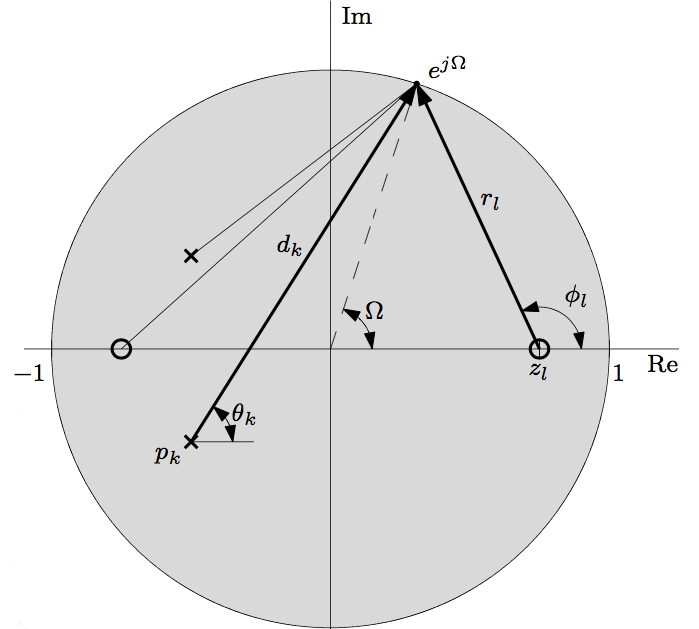
\includegraphics[width=\linewidth]{lathi}
 \captionof{figure}{Los polos y los ceros determinan $H(z)$}
 \label{fig:circulo}
\end{figurehere}

\subsection{Método 2} % SI APLICA
\lipsum[7]
Se puede encontrar una demostración detallada en \cite{Sh:575} , \cite{Sh:572}.
\subsection{Método 3} % SI APLICA
\
\lipsum[8] En \cite{webster} se puede ver que:

\begin{equation}
 e^{ \ j  \pi} = -1
 \label{euler}
\end{equation}
La ecuancion \ref{euler} es conocida como la identidad de Euler.
